\section{Metamodel requirements}
\label{sec:requirements}
The requirements [RX] formulation process for MeROS metamodel is multi-stage and iterative. In the beginning, the initial requirements were formulated based on: (i) literature review (both scientific and ROS wiki/community sources), (ii) author experience from supervising and supporting ROS-based projects, and finally, (iii) author experience from EARL (Embodied Agent-based cybeR-physical control systems modelling Language)~\cite{earl2020} PIM development and its applications (e.g.~\cite{tasker2020,karwowski2021hubero,en14206693-grav-comp}). Verification of subsequent versions of MeROS by its practical applications led to an iterative reformulation of requirements and MeROS itself.

MeROS requirements are depicted on a~number of dedicated SysML diagrams. The requirements are organised in a~tree-like nesting structure, with additional internal relations, and labelled following this structure. The general requirements are presented in Fig.~\ref{fig:general_req}. Here, and in the following diagrams, the elements (components, relations) specific for a particular version of ROS (ROS~1 or ROS~2) are labelled with an ,,rv''  tag with the ROS version that the element is specific for. The lack of a tag means the element is general for both ROS versions.


\begin{figure}[H]
	\centering
	\begin{center}
	{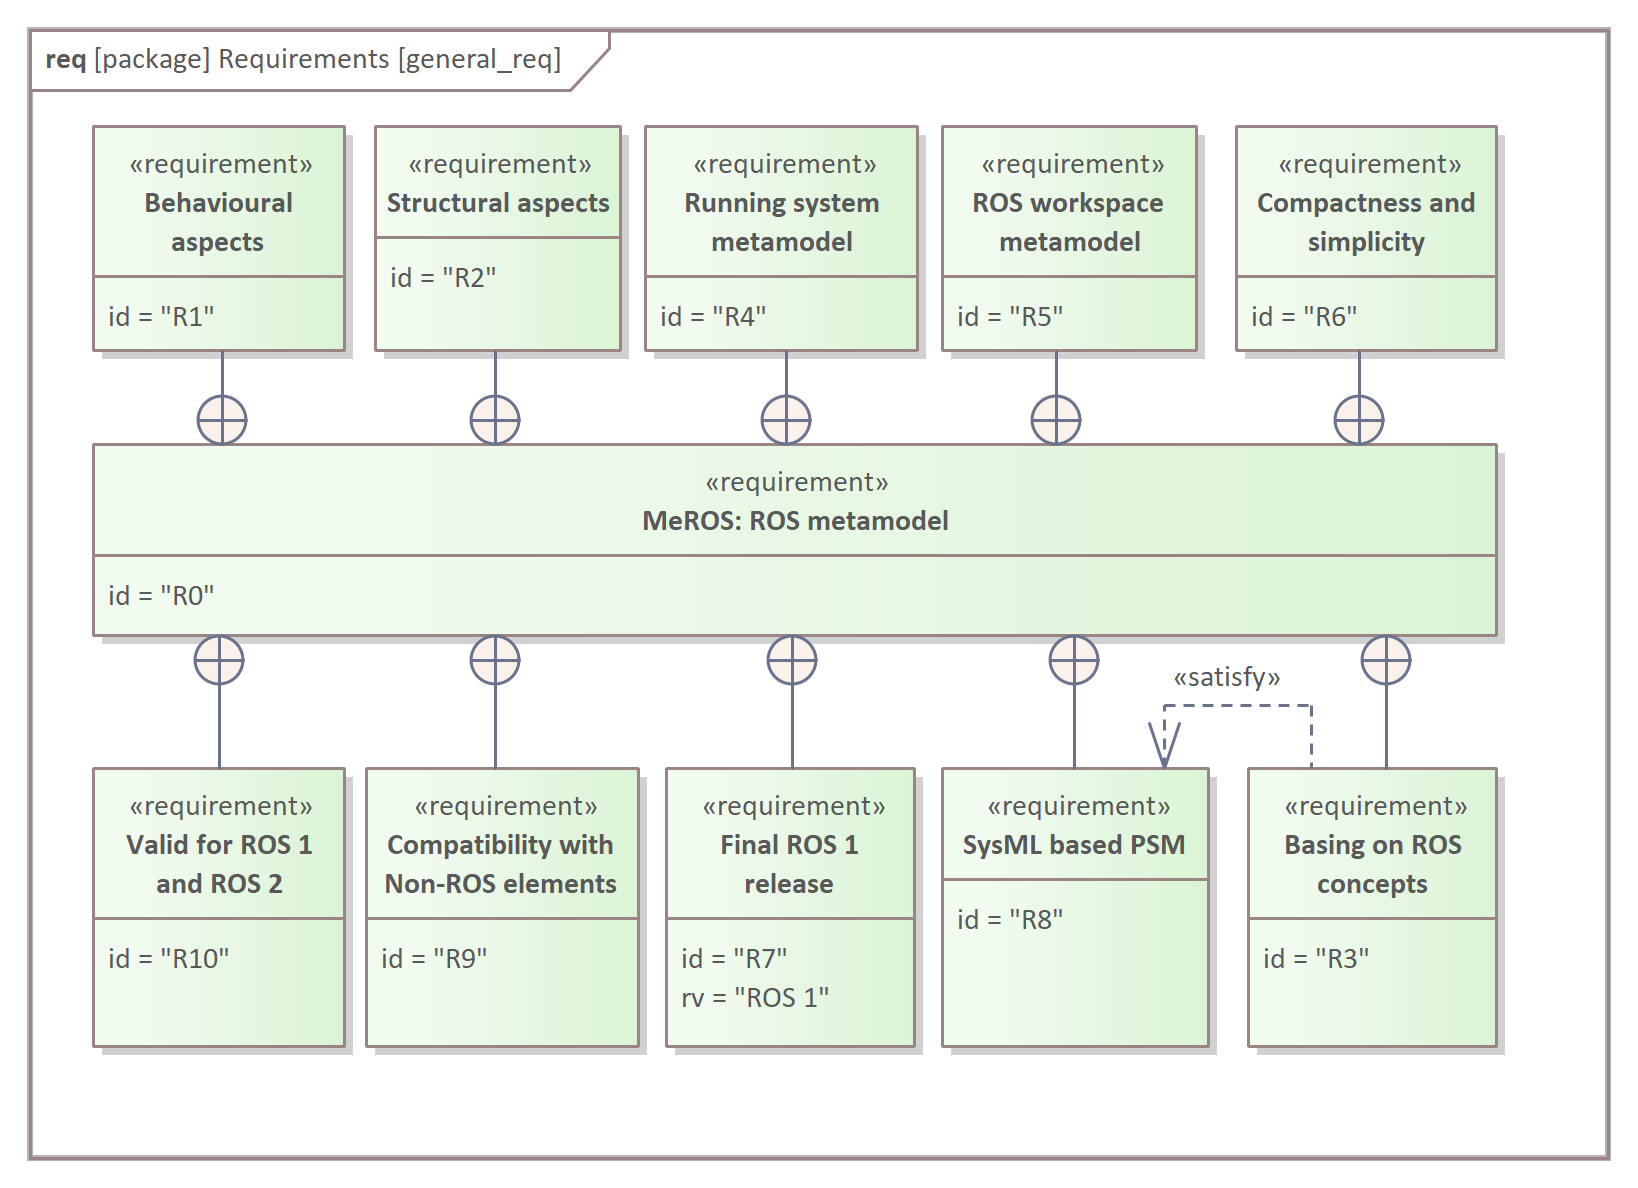
\includegraphics[scale=0.9]{../imgs/requirement_pkg/general_req.png}}
	\end{center}
	\caption{General requirements.}
	\label{fig:general_req}
\end{figure}


The SysML models have two main parts: behavioural [R1] and structural [R2]. MeROS aims to cover ROS concepts [R3] and not change their labels as long as possible, to maintain conformity and intuitiveness. The ROS system is two-faced. While it is executed [R4], it has a~specific structure and behaviour, but from the developers' point of view, the workspace [R5] is the exposed aspect. The model should be compact and straightforward [R6] rather than unnecessarily elaborate and complicated. One of the assumptions that stand out MeROS from other ROS metamodels is conformity with the final ROS~1 release [R7] (Noetic Ninjemys). Although the SysML-based MeROS is classified into PSM [R8], it should be compatible with Non-ROS elements [R9]. Finally, MeROS metamodel should be valid both for ROS~1 and ROS~2.

The system's structural aspects requirements are presented in Fig.~\ref{fig:structural_aspects_req}.

\begin{figure}[H]
	\centering
	\begin{center}
	{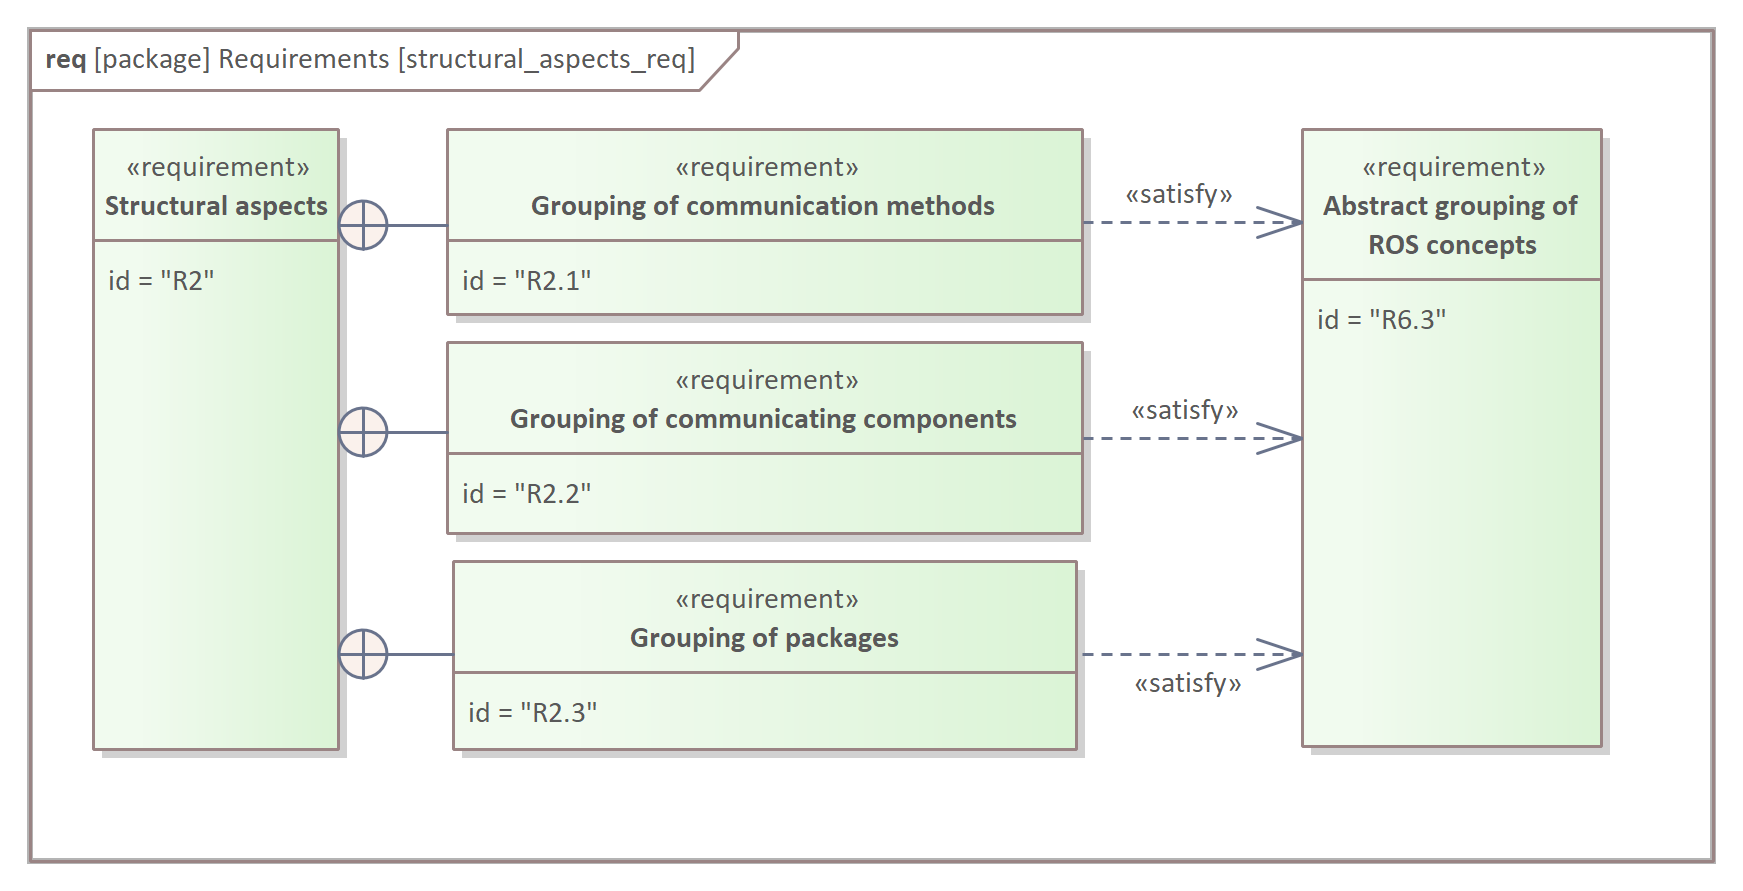
\includegraphics[scale=0.9]{../imgs/requirement_pkg/structural_aspects_req.png}}
	\end{center}
	\caption{Structural aspects requirements.}
	\label{fig:structural_aspects_req}
\end{figure}

A~vital addition to the original ROS concepts is the abstract grouping of: (i) communicating methods [R2.1] and (ii) communicating components [R2.2]. The motivation for the introduction of these aggregates is presented further on. It should be noted that several ROS concepts group other concepts in a particular way, especially to deploy the system. Action aggregates Topics and Services (in ROS~2), ROS~1 Node aggregates Nodelets, and ROS~2 Component Container aggregates Nodes.
The ROS concepts that MeROS models are organised into four major classes (Fig.~\ref{fig:ros_concepts_req}): (i) Communicating components [R3.1], (ii) Communication methods [R3.2], (iii) Workspace [R3.3], and (iv) Other [R3.4].


\begin{figure}[H]
	\centering
	\begin{center}
	{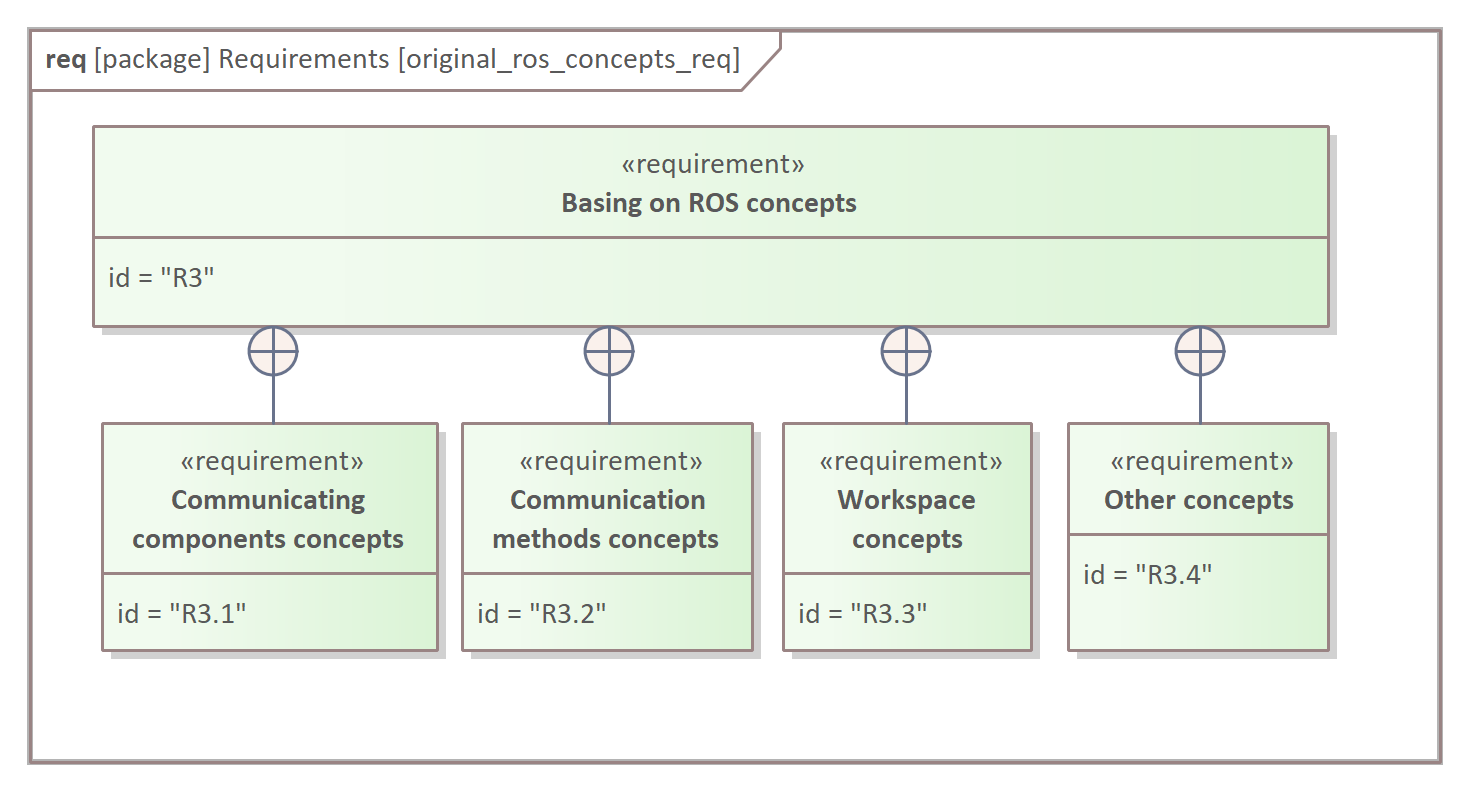
\includegraphics[scale=1.1]{../imgs/requirement_pkg/original_ros_concepts_req.png}}
	\end{center}
	\caption{ROS concepts requirements.}
	\label{fig:ros_concepts_req}
\end{figure}

Communicating components [R3.1] are: (i) ROS Node, (ii) ROS Nodelet, (iii) ROS plugin, and (iv) ROS library. Both plugin and library let to share the same code between various Nodes or ROS~1 specific Nodelets. Two ROS nodes are mandatory to execute the ROS~1 system: (i) ROS Master and (ii) rosout.

\begin{figure}[H]
	\centering
	\begin{center}
	{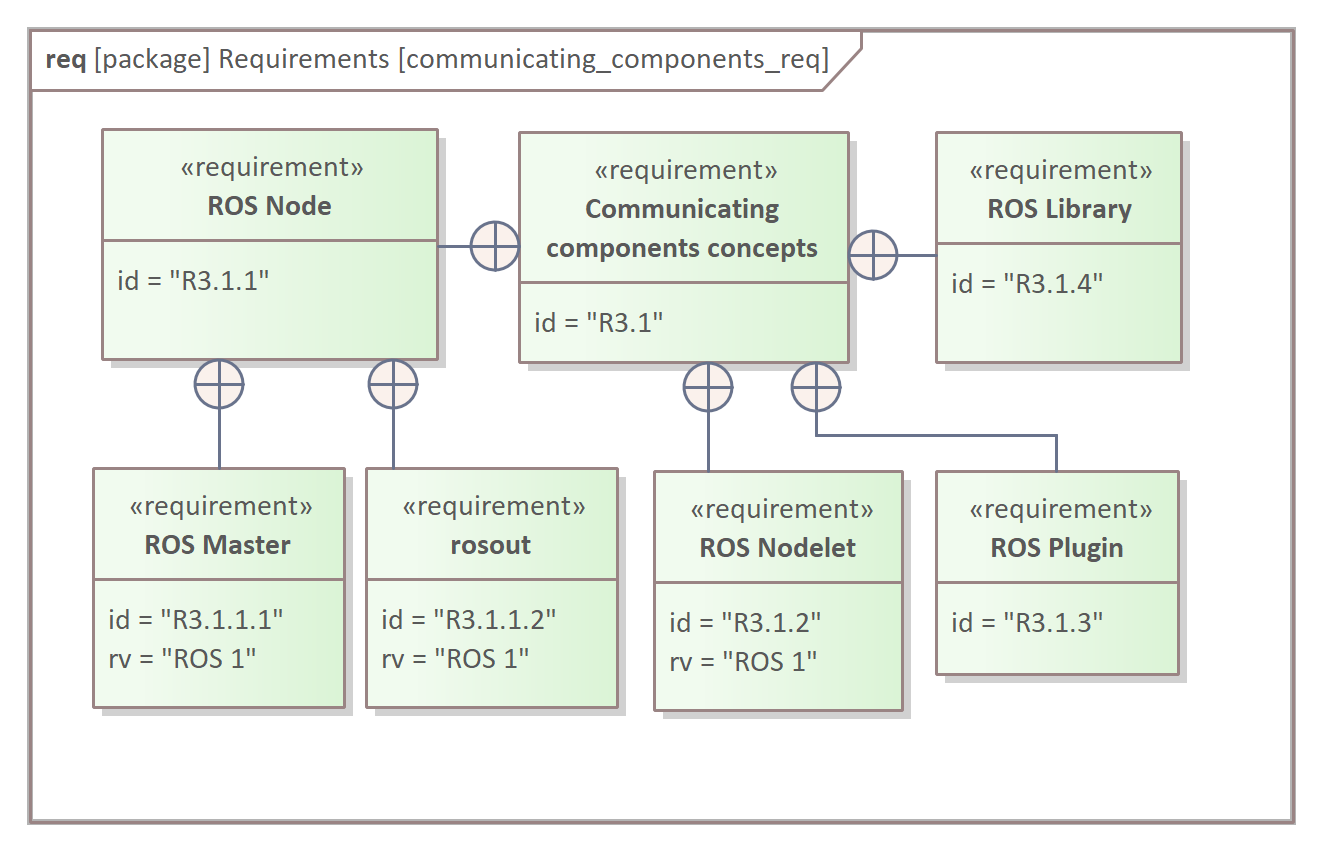
\includegraphics[scale=1]{../imgs/requirement_pkg/communicating_components_req.png}}
	\end{center}
	\caption{Communicating components requirements.}
	\label{fig:communicating_components_req}
\end{figure}
Communication methods are depicted in Fig.~\ref{fig:communication_concepts_req}.
Three methods of communication are considered [R3.2] with their inter-component connections and data structures: (i) ROS Topic, its Message and connection, (ii) ROS Service comprising data structure and connection, and finally (iii) ROS Action including data structure and connection.

\begin{figure}[H]
	\centering
	\begin{center}
	{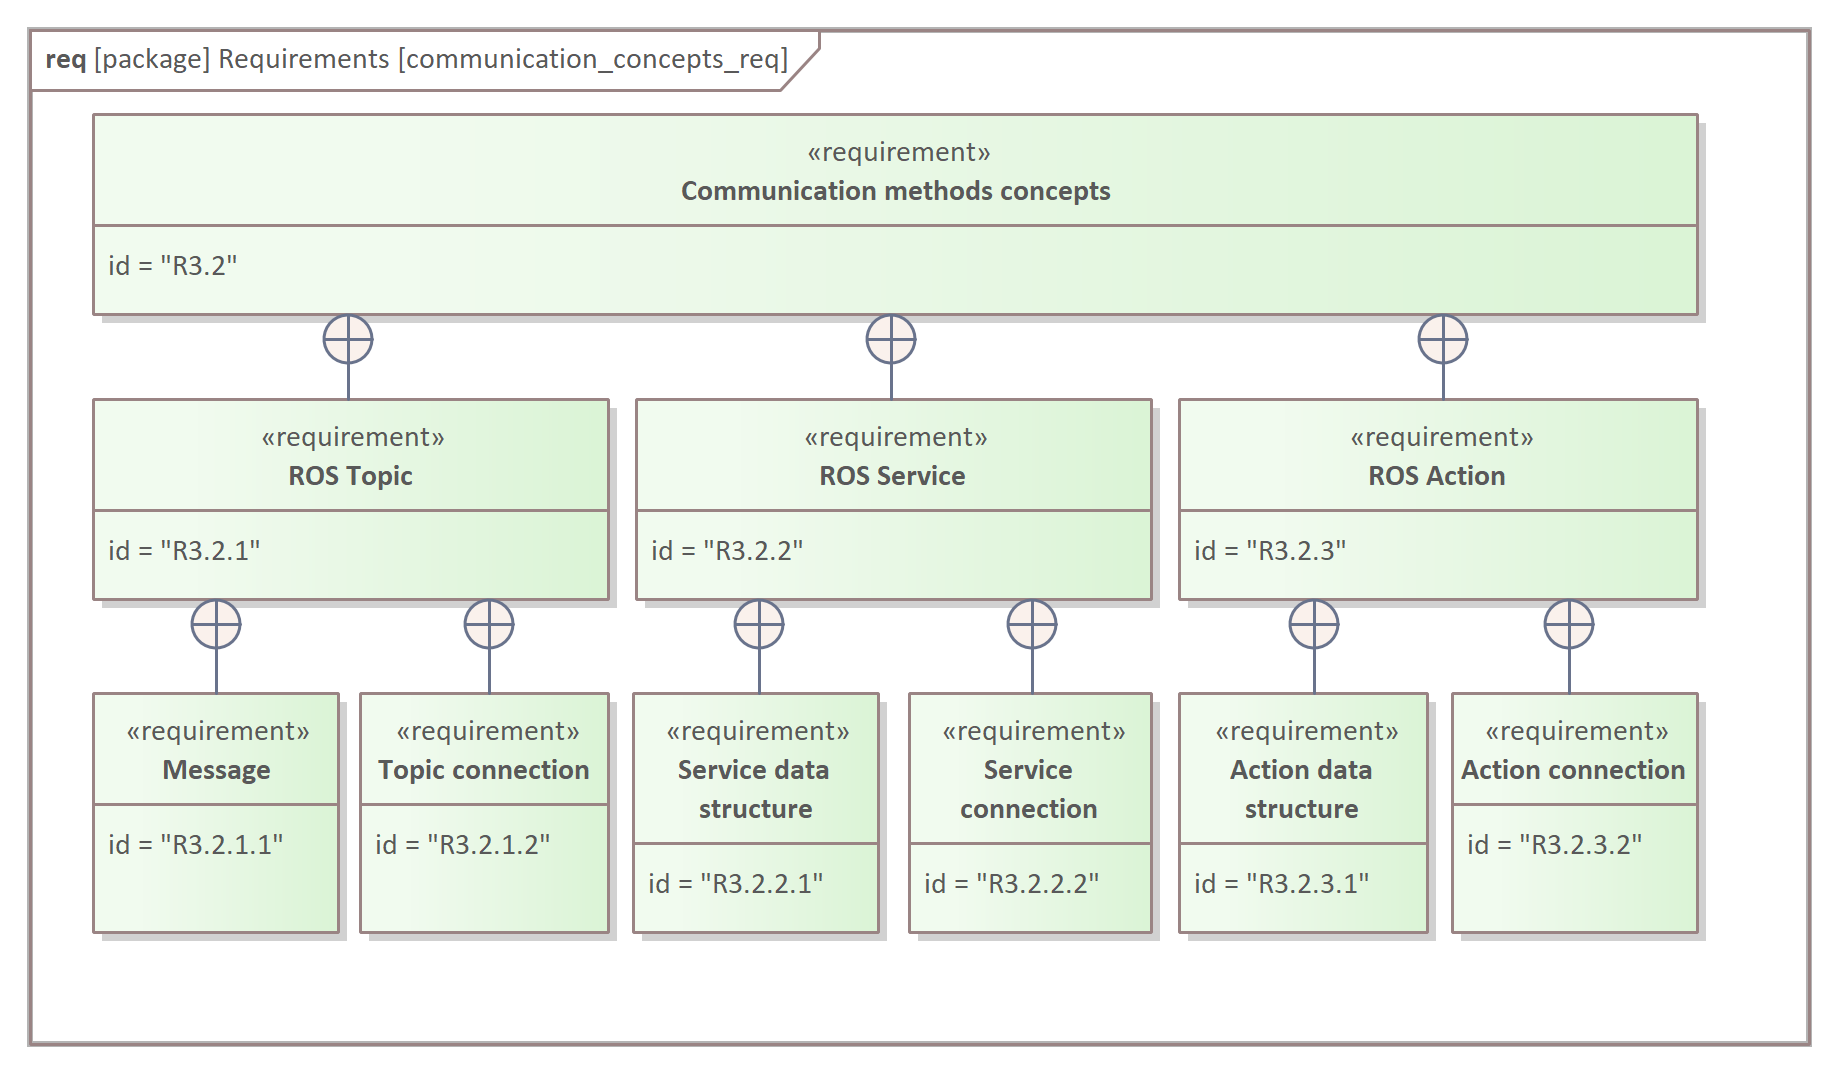
\includegraphics[scale=1]{../imgs/requirement_pkg/communication_concepts_req.png}}
	\end{center}
	\caption{Communication concepts requirements.}
	\label{fig:communication_concepts_req}
\end{figure}
Workspace concept [R3.3] comprises: (i) ROS Package [R3.3.1], (ii) Metapackage [R3.3.2] introduced in the latest releases of ROS~1, (iii) Group of packages [R3.3.3], (iv) Repository [R3.3.4] and (v) ROS Workspace [R3.3.5].

\begin{figure}[H]
	\centering
	\begin{center}
	{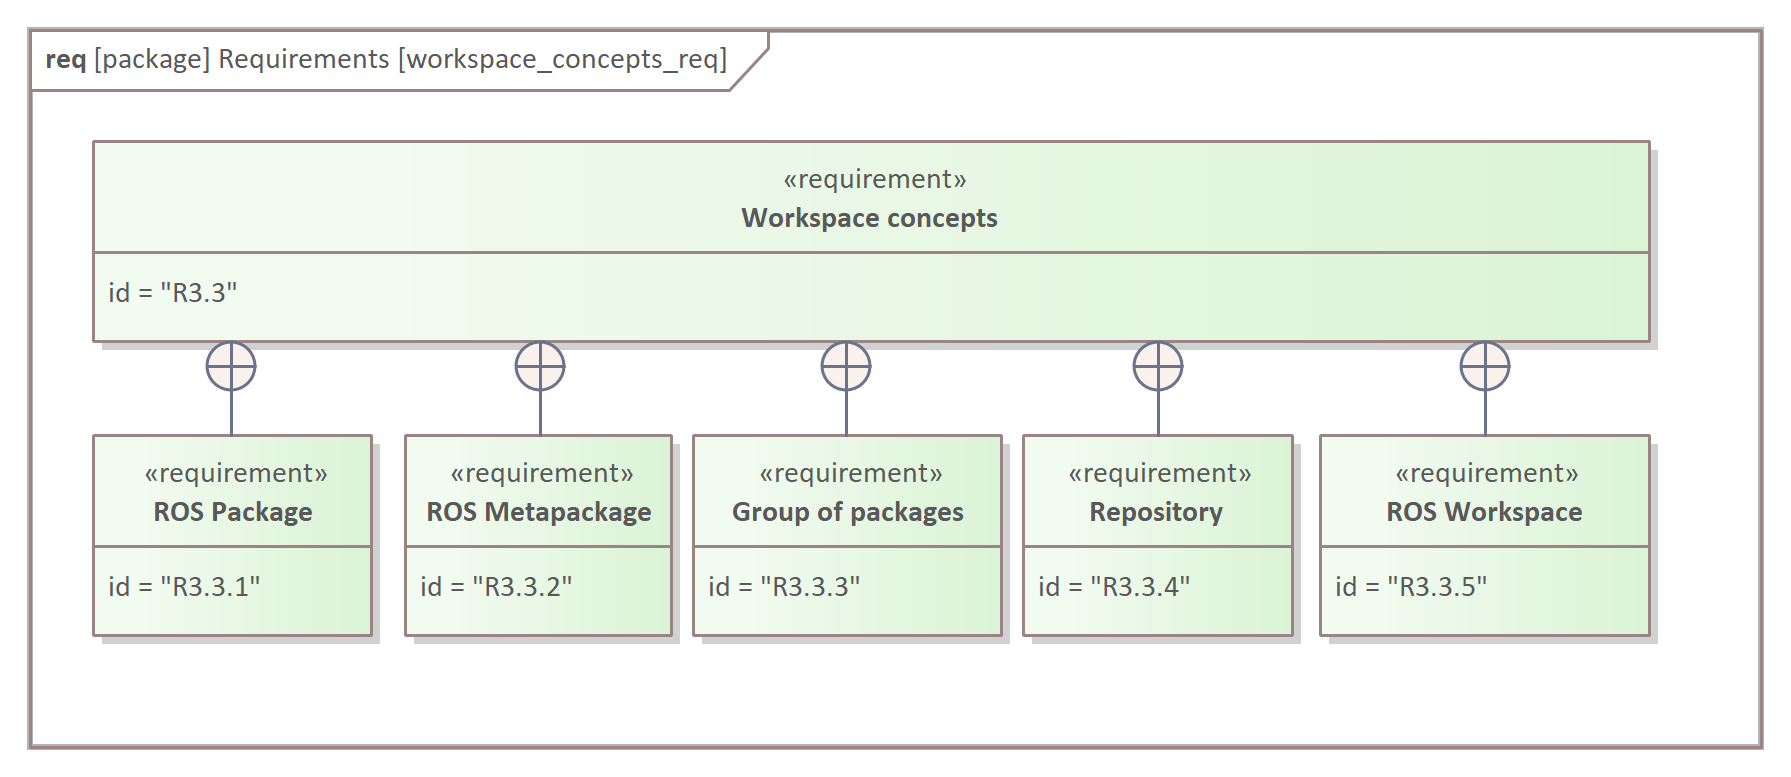
\includegraphics[scale=1]{../imgs/requirement_pkg/workspace_concepts_req.png}}
	\end{center}
	\caption{Workspace concepts requirements.}
	\label{fig:workspace_concepts_req}
\end{figure}

\pagebreak

Other concepts (Fig.~\ref{fig:other_concepts_req}) [R3.4] include four elements: (i) ROS Parameter Server manages (ii) ROS Parameters, (iii) roscore forms a collection of programs and nodes that are pre-requisites of a ROS~1-based system. Finally, (iv) ROS Namespace reflects the ROS concept to organise nodes and communication connections. Both ROS Master and rosout are executed with roscore. ROS Parameter Server is a part of ROS Master.

\begin{figure}[H]
	\centering
	\begin{center}
	{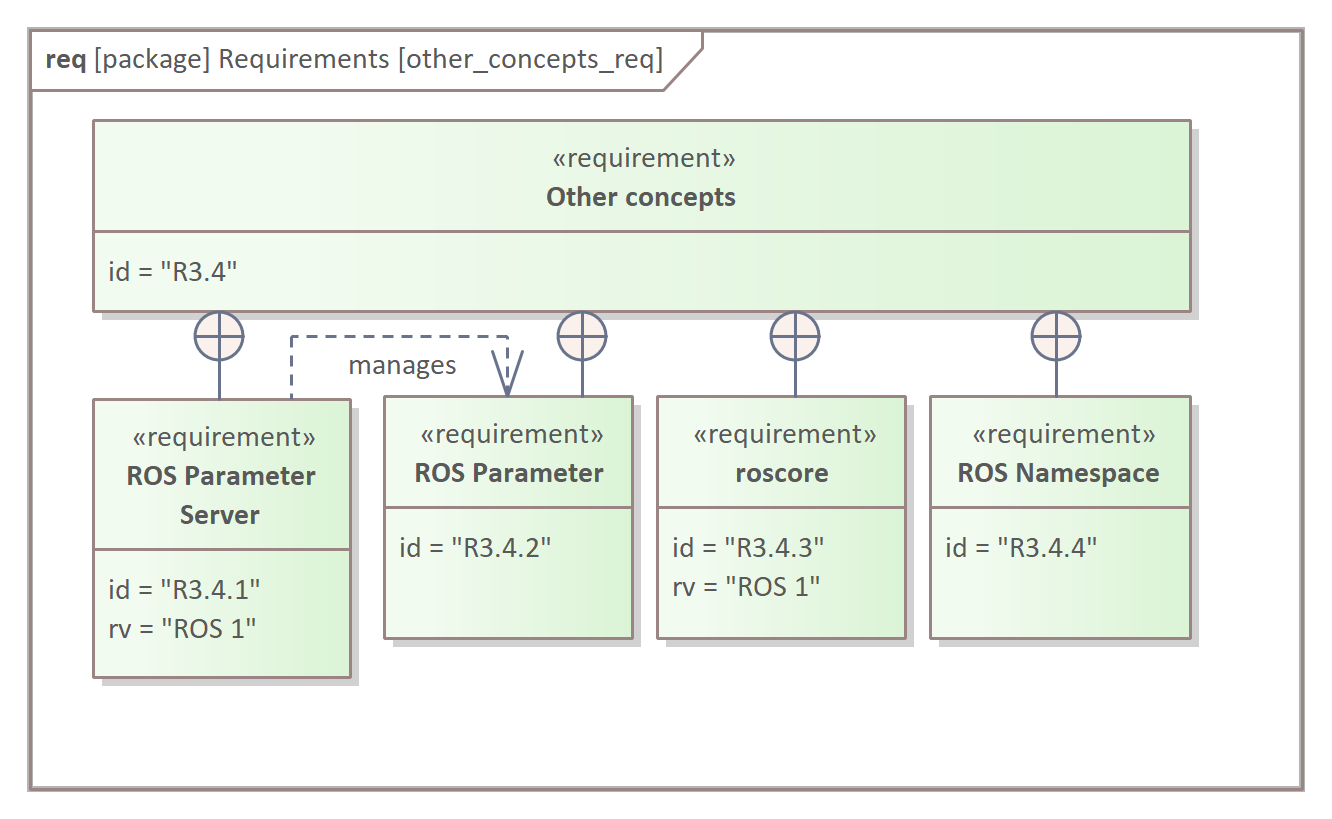
\includegraphics[scale=1.1]{../imgs/requirement_pkg/other_concepts_req.png}}
	\end{center}
	\caption{Other ROS concepts requirements.}
	\label{fig:other_concepts_req}
\end{figure}

Fig.~\ref{fig:roscore_req} presents additional roscore-related relations.


\begin{figure}[H]
	\centering
	\begin{center}
	{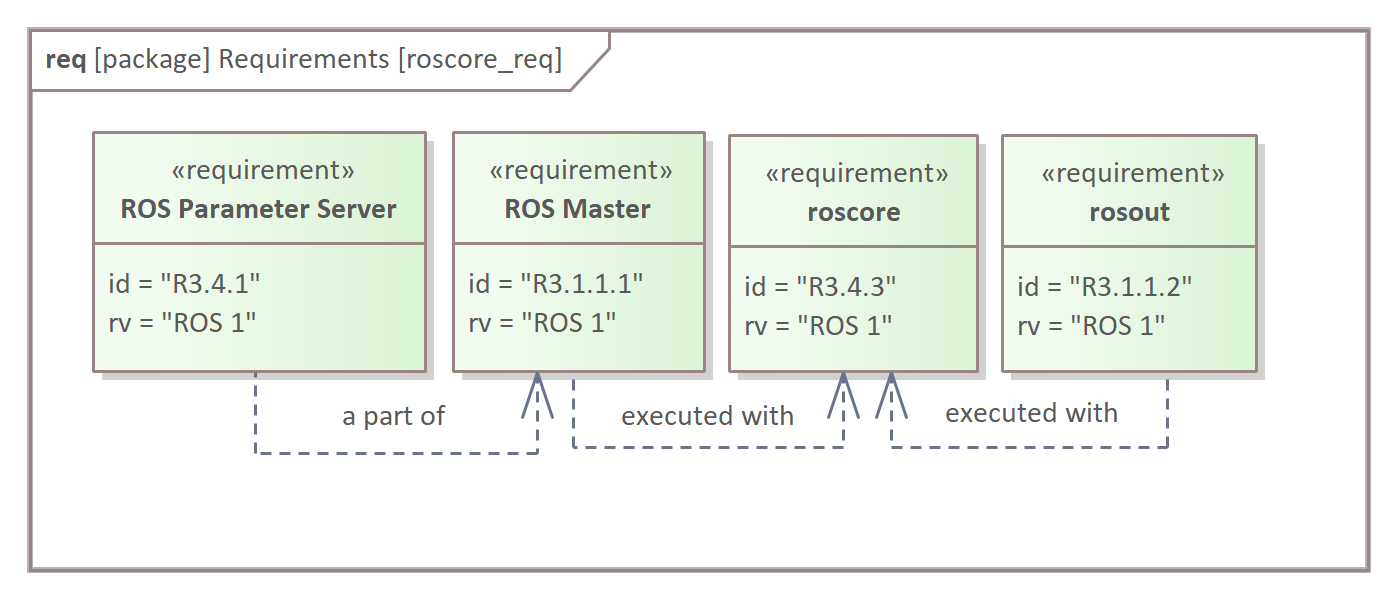
\includegraphics[scale=1.1]{../imgs/requirement_pkg/roscore_req.png}}
	\end{center}
	\caption{roscore related requirements dependences.}
	\label{fig:roscore_req}
\end{figure}

\pagebreak

To achieve intuitiveness, MeROS presents a Running system structure (Fig.~\ref{fig:running_system_req}) following ROS rqt\_graph pattern [R4.1]. In particular, there are two ways to visualise communication, including [R4.1.1] and without [R4.1.2]
dedicated communication components.
\begin{figure}[H]
	\centering
	\begin{center}
	{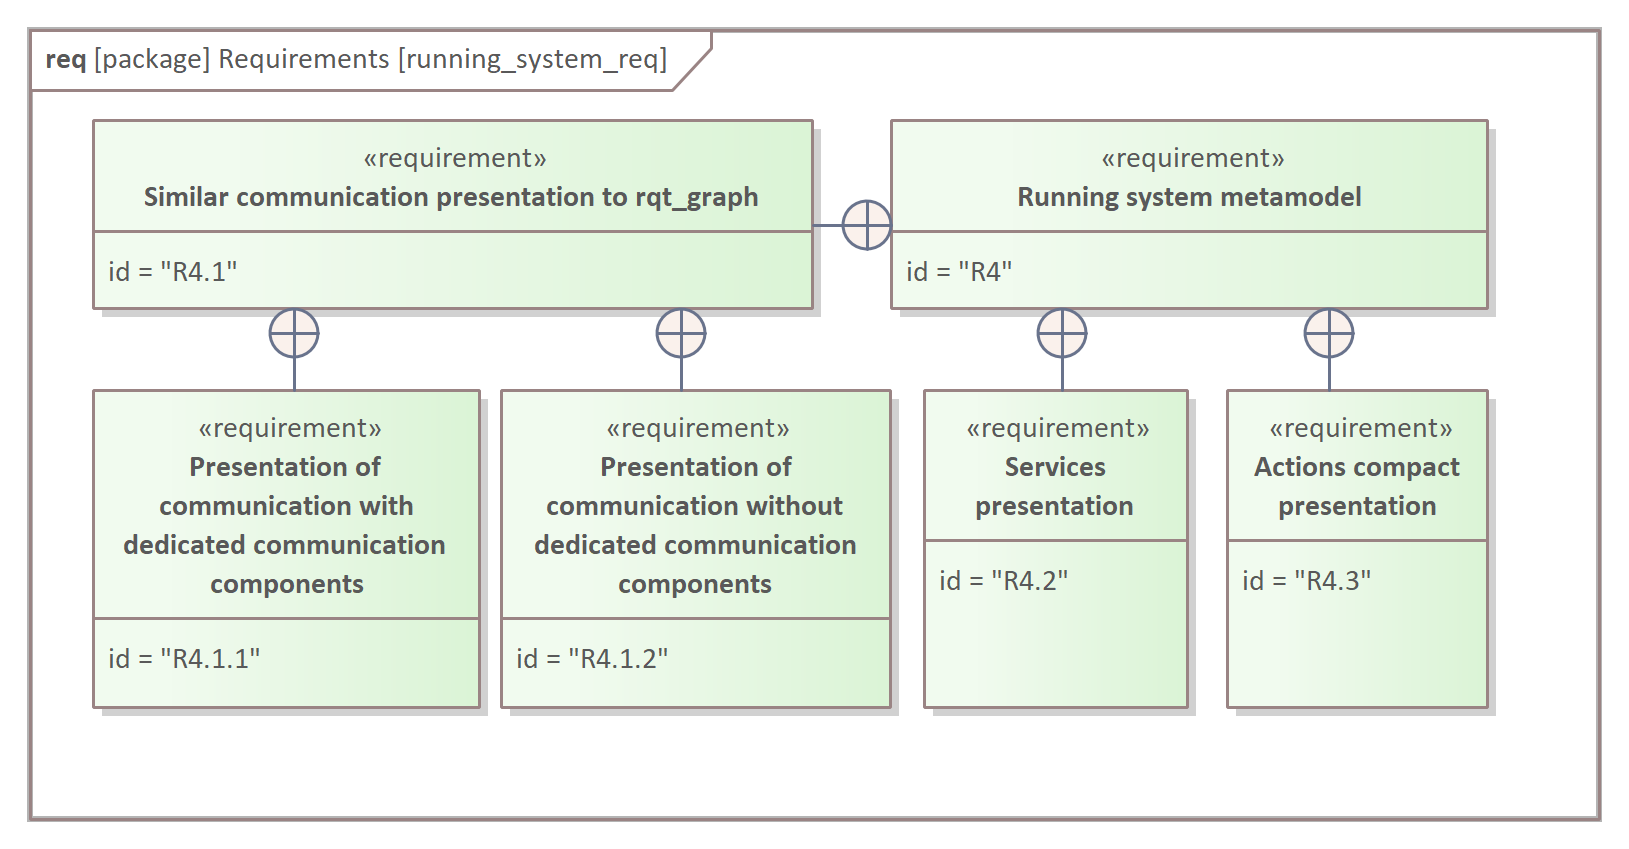
\includegraphics[scale=0.9]{../imgs/requirement_pkg/running_system_req.png}}
	\end{center}
	\caption{Running system requirements.}
	\label{fig:running_system_req}
\end{figure}
The dedicated components are especially useful in the presentation when many communication components use the same topic both on the publisher and the subscriber side. In opposition, the expression of topic names on arrows connecting communicating components, i.e., without dedicated communication components, let to reduce the number of components needed to depict communication for many topics and a~low number of communicating components. The other advantage of using dedicated communication components is that the particular connection can be split into several diagrams (e.g. ibd (internal block diagram) or sd (sequence diagram)), where the same object represents this connection in every associated diagram. Services [R4.2] and actions [R4.3] should be depicted as an addition to the presentation of the particular topics. It should be noted that rqt\_graph represents actions as a~number of topics and services. In MeROS, the topics and services being part of an action can be aggregated, which reduces the number of depicted connections.


The compactness and simplicity [R6] and its nesting requirements are presented in Fig.~\ref{fig:compactness_and_simplicity_req}.

\begin{figure}[H]
	\centering
	\begin{center}
	{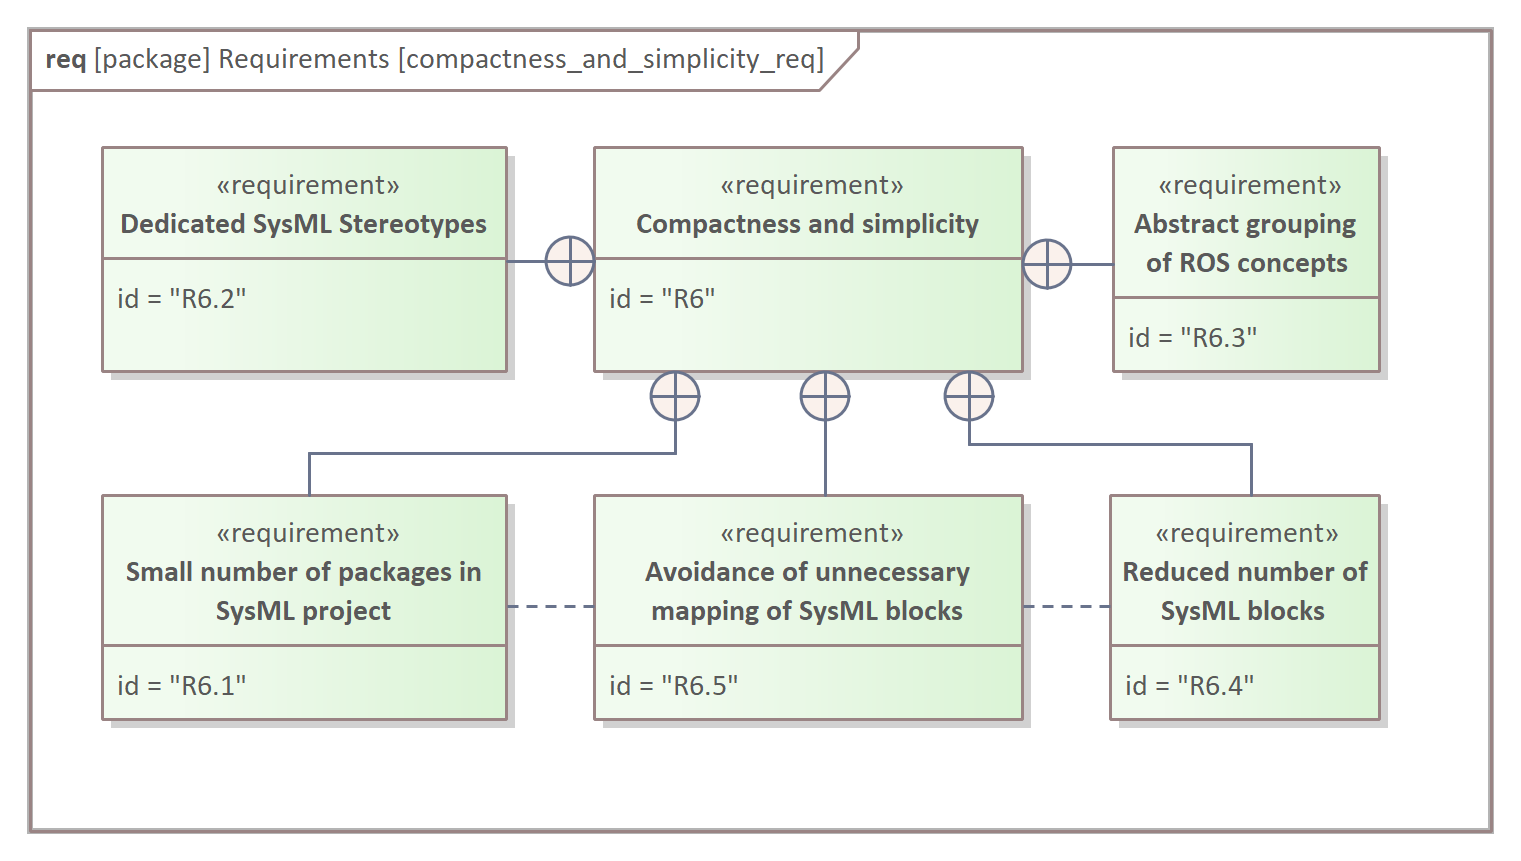
\includegraphics[scale=0.9]{../imgs/requirement_pkg/compactness_and_simplicity_req.png}}
	\end{center}
	\caption{Compactness and simplicity requirements.}
	\label{fig:compactness_and_simplicity_req}
\end{figure}

A SysML project to develop and represent MeROS metamodel should consist of a~small number of packages [R6.1], but still, the packages should distinguish the major aspects of development process: (i) metamodel requirements formulation, (ii) metamodel itself, and (iii) metamodel realizations/applications.
Dedicated SysML stereotypes [R6.2] are introduced to MeROS to replace the direct block specialization representation on diagrams and improve the legibility and compactness of diagrams.
The grouping of concepts [R6.3] has diverse aims. It enables the presentation of the system part in a~general, PIM-like abstract way, on the logical level rather than a~detailed, PSM-like implementation one. The aggregation reduces the number of objects represented on the diagram to highlight the essential aspects and stay compact and consistent in presentation.
The number of SysML blocks should be reduced to a reasonable level [R6.4]. Both [R6.1] and [R6.4] help in the Avoidance of unnecessary mapping of SysML blocks [R6.5].

There are three elements in the requirements set that satisfy the evolution of the ROS~1  finalised with its ultimate release -- Noetic Ninjemys -- (Fig.~\ref{fig:final_ros1_release_req}): (i) ROS Nodelet  (introduced primarily to increase the efficiency of ROS components switching), (ii) ROS Action , and (iii) ROS Metapackage.

\begin{figure}[H]
	\centering
	\begin{center}
	{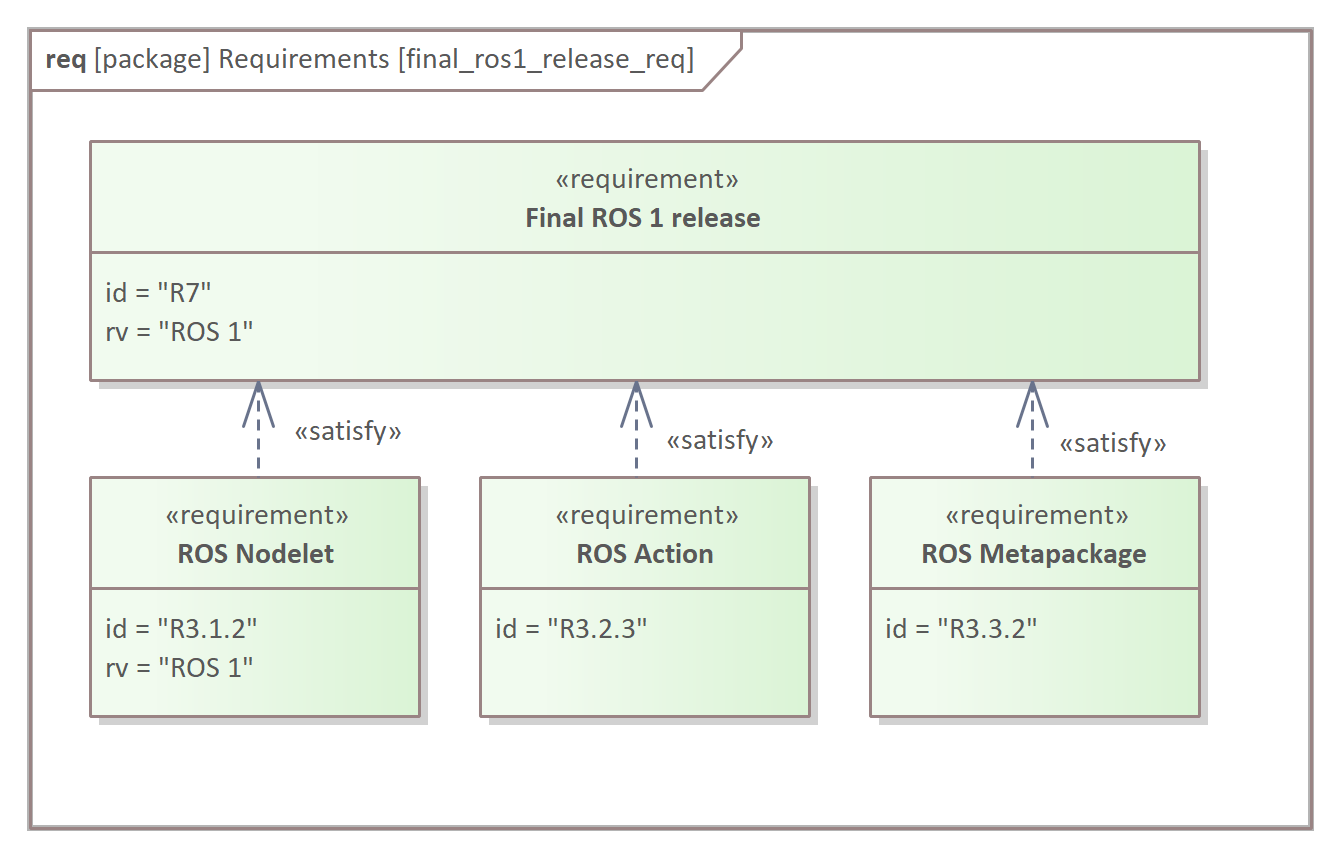
\includegraphics[scale=1.1]{../imgs/requirement_pkg/final_ros1_release_req.png}}
	\end{center}
	\caption{Final ROS 1 release requirements.}
	\label{fig:final_ros1_release_req}
\end{figure}
